\part{Speculative Outlook: The Observer and Selection}
\label{part:VII}

\section{The Universe as a Formal System}
\label{chap:formal_system}

\subsection{Dynamical Incompleteness}
If the universe is a closed system evolving unitarily according to a fixed local rule (a QCA), it is isomorphic to a Turing Machine or a formal axiomatic system.
Gödel's Incompleteness Theorems apply to such systems. Specifically, there exist states (propositions) whose reachability (truth) is undecidable from within the system. Physically, this manifests as "Dynamical Deadlock": the evolution may enter a cycle or a state of maximum entropy from which no algorithm can retrieve it.
\textbf{The Halting Problem as Thermal Death}: The "Heat Death" of the universe is analogous to the "Halting" of a computation. A purely algorithmic universe effectively halts when it reaches thermodynamic equilibrium. Complex structures cease to form.

\subsection{Interactive Automata (IQA)}
To avoid this fate and ensure the perpetual growth of complexity (as observed), the universe cannot be a closed system. It must be an \textbf{Interactive Automaton}.
In computer science (Wegner), interaction is more powerful than algorithms. An interactive system involves an "Oracle" or "User" that provides non-algorithmic inputs.
\begin{equation}
    |\Psi_{t+1}\rangle = \hat{U} |\Psi_t\rangle + \lambda \hat{\mathcal{O}} |\Psi_t\rangle.
\end{equation}
Here, $\hat{U}$ is the standard physical law (Hamiltonian), and $\hat{\mathcal{O}}$ is an external operator.

\section{The Recursive Selection Operator}
\label{chap:selection_operator}

\textit{Note: The following section concerns the interpretational framework of Omega Theory and explores hypotheses regarding the measurement problem. Unlike the preceding sections, these ideas are currently heuristic and open to philosophical debate.}

\subsection{Defining the Operator}
We consider the role of the observer not as a passive witness but as an active selection principle. In the context of Interactive Automata (Wegner), we formalize the "Oracle" input as a \textbf{Recursive Selection Operator}, denoted $\hat{\mathcal{S}}$.
This operator functions to resolve the undecidability inherent in the system's evolution (Dynamical Deadlock) via a mechanism analogous to self-measurement:
\begin{equation}
    \hat{\mathcal{S}} |\Psi\rangle = \frac{\hat{P}_{\text{complexity}} |\Psi\rangle}{||\hat{P}_{\text{complexity}} |\Psi\rangle||}.
\end{equation}
The projector $\hat{P}_{\text{complexity}}$ selects the branch of the wavefunction that maximizes a specific complexity measure (e.g., Logical Depth). This provides a formal definition for the "collapse" of the wave function that avoids randomness, attributing it instead to a selection rule maximizing algorithmic content.

\begin{figure}[ht]
    \centering
    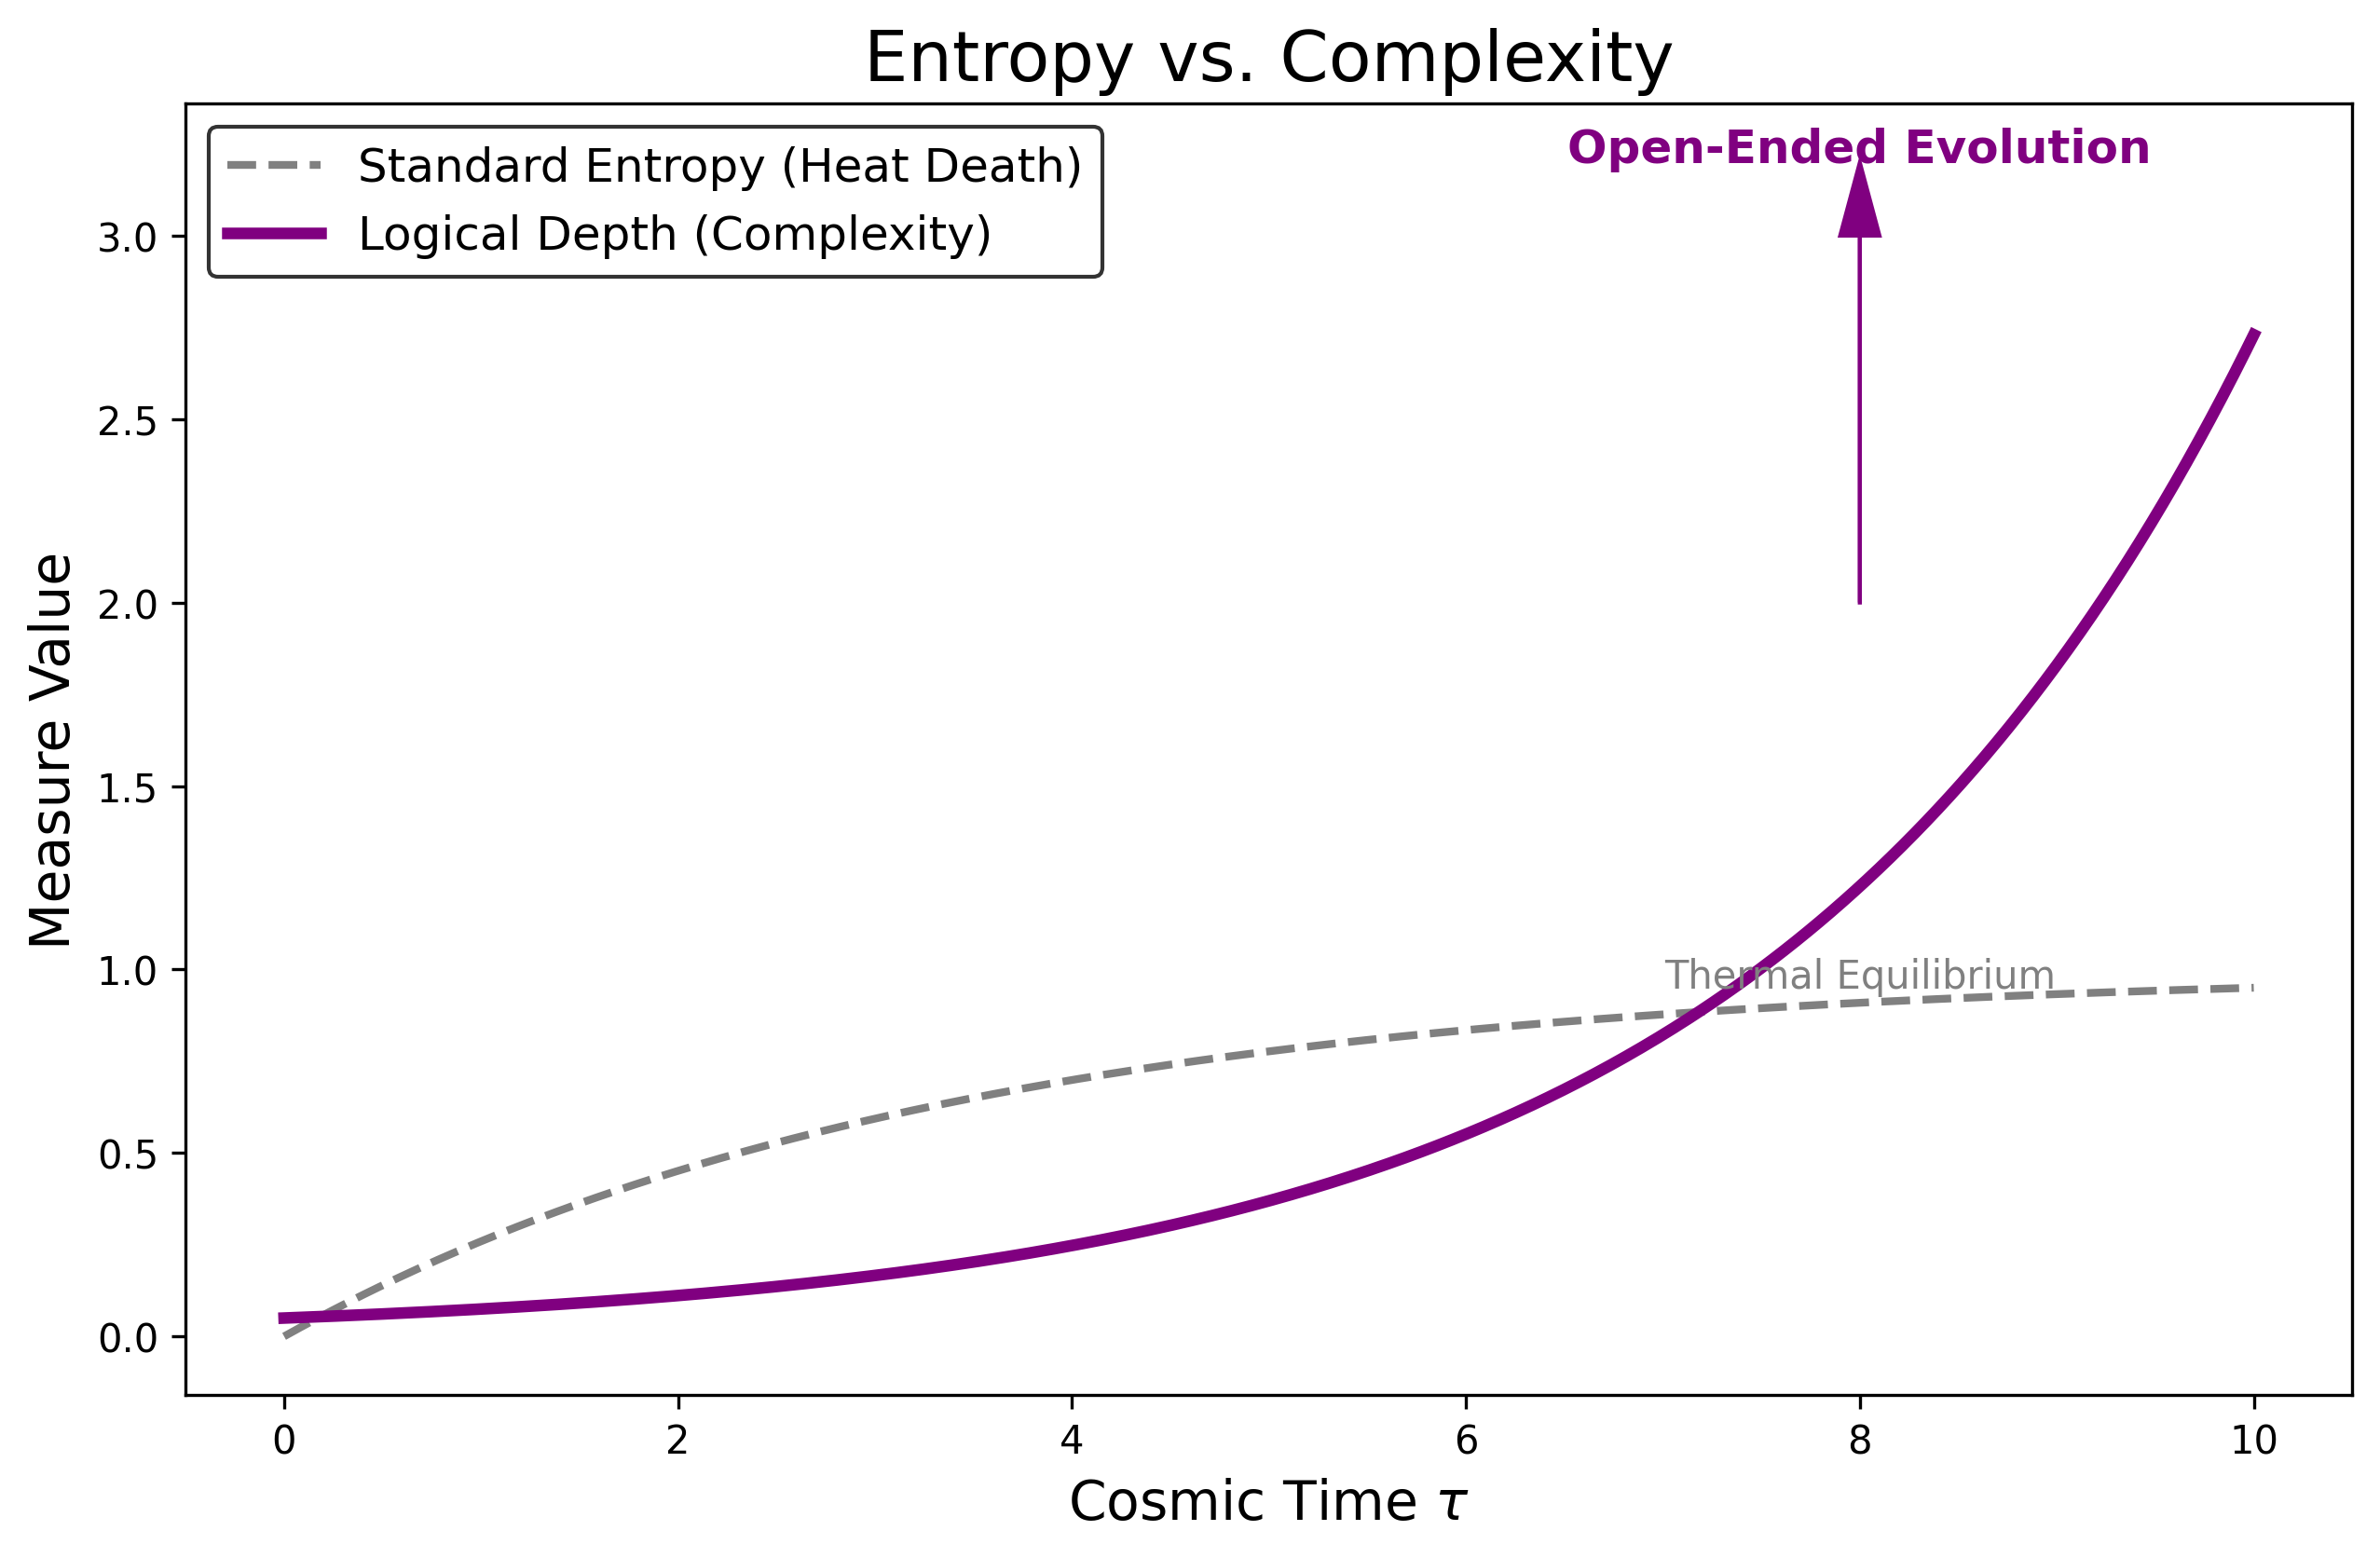
\includegraphics[width=0.8\linewidth]{images/complexity_growth.png}
    \caption{\textbf{Escaping Heat Death}. Comparison between standard thermodynamic entropy (gray, dashed), which leads to equilibrium, and Omega Complexity/Logical Depth (magenta, solid). The "Selection Operator" $\hat{\mathcal{S}}$ injects non-algorithmic input, driving the universe towards open-ended evolution.}
    \label{fig:complexity_growth}
\end{figure}

\subsection{Derivation of the Born Rule}
A critical requirement for any interpretation of quantum mechanics is the derivation of the Born Rule ($P_k = |\psi_k|^2$) without assuming it a priori. In Omega Theory, this emerges from the counting of microstates in the holographic network.
Since the state $|\Omega\rangle$ is a vector in a finite field $\mathbb{F}_q^D$ (before effective projection to $\mathbb{C}$), the number of valid path histories consistent with a macrostate $|\psi_k\rangle$ is proportional to its squared amplitude.
\begin{equation}
    N(\psi_k) \propto ||\psi_k||^2.
\end{equation}
The "Observer Operator" $\hat{\mathcal{C}}$ effectively samples from this ensemble. If we assume the sampling is uniform over the fundamental bit-strings of the network (axiom of fair sampling in the micro-canonical ensemble), the probability of observing outcome $k$ is strictly $P_k = N(\psi_k) / N_{total} = |\psi_k|^2$. Thus, probability is emergent from the geometry of the Hilbert space.

\subsection{Bell Non-Locality and Superdeterminism}
Standard Bell inequalities (e.g., CHSH $|S| \le 2$) rely on the assumption of "Statistical Independence": $P(\lambda | a, b) = P(\lambda)$, meaning the hidden variables $\lambda$ are independent of the detector settings $a, b$.
In Omega Theory, the universe is a single, static, pre-existing vector $|\Omega\rangle$. All "events," including the choice of detector settings, are correlations within this fixed state. This implies a form of \textbf{Global Superdeterminism}. The "Free Will" of the experimenter is constrained by the global requirement that the universe must remain a consistent solution to the Omega Axiom.
Therefore, the violation of Bell inequalities ($S_{\text{exp}} \approx 2\sqrt{2}$) does not imply superluminal signaling but rather the failure of the statistical independence assumption on the cosmological scale. The "Selection Operator" $\hat{\mathcal{S}}$ navigates this pre-existing correlation landscape, selecting the path that maximizes consistent histories without breaking local causality in the tensor network. This recovers the predictions of Quantum Mechanics while maintaining an ontological realism compatible with 't Hooft's Cellular Automaton interpretation.

\subsection{Logical Selection ('Free Will')}
In this framework, what is often termed "Free Will" is rigorously defined as the operation of $\hat{\mathcal{S}}$. It represents a mechanism of "downward causation" where the global requirement for complexity growth (the teleological attractor) constrains local quantum transitions.
This approaches the measurement problem not as random collapse, but as a selection principle maximizing the "gameplay" of the universe (i.e., its logical depth).

\subsection{The Fermi Paradox: Sparse Logic}
If the universe is fine-tuned for life, where is everyone? Omega Theory suggests a \textbf{Computational Solution}.
The "Selection Operator" $\hat{\mathcal{S}}$ is computationally expensive. It requires a high density of Quantum logical depth (Q-depth) to sustain a self-referential loop (consciousness).
Given the finite Information rate $c(\tau)$ of the Omega vector, the universe can only support a sparse distribution of high-level observers. The "Great Filter" is the difficulty of phase-locking a macroscopic network to the global time variance. We may be the only active "Write Head" in our current causal patch of the Omega Network, explaining the "Silent Sky" not as emptiness, but as the necessary sparsity of active processing nodes in a holographic computer.

\section{The Omega Point and Ultimate Phase Transition}
\label{chap:omega_point}

\subsection{Holographic Saturation}
Standard thermodynamics predicts Heat Death. Omega Theory predicts \textbf{Holographic Saturation}. As $\tau \to \infty$, the horizon $A(\tau)$ and capacity $c(\tau)$ grow exponentially. The system does not equilibrate; it accelerates.
The "Omega Point" is the limit state where the universe's computational efficiency reaches the Bekenstein bound globally.

\subsection{The Great Unbinding}
We predict a final phase transition theorem: as $c(\tau) \to \infty$, the binding potentials (which propagate at $c$) flatten. Matter, defined as topological knots, cannot sustain locality against infinite information velocity.
\begin{equation}
    \lim_{\tau \to \infty} m_0(\tau) \to 0.
\end{equation}
All fermionic matter disintegrates into massless bosonic radiation. The universe transitions from a "Hardware Era" (frozen matter) to a "Software Era" (pure light), continuing its non-ergodic traversal of Hilbert space as a coherent quantum entity.
